%\documentclass{ExcelAtFIT}
\documentclass[czech]{ExcelAtFIT} % when writing in CZECH
%\documentclass[slovak]{ExcelAtFIT} % when writing in SLOVAK


\makeatletter
\setlength{\@fptop}{0pt}
\makeatother

%--------------------------------------------------------
%--------------------------------------------------------
%	REVIEW vs. FINAL VERSION
%--------------------------------------------------------

%   LEAVE this line commented out for the REVIEW VERSIONS
%   UNCOMMENT this line to get the FINAL VERSION
\ExcelFinalCopy


%--------------------------------------------------------
%--------------------------------------------------------
%	PDF CUSTOMIZATION
%--------------------------------------------------------

\hypersetup{
	pdftitle={Detekce dopravních značek v obraze a videu pomocí konvolučních neuronových sítí},
	pdfauthor={Filip Kočica},
	pdfkeywords={Konvoluční neuronová síť --- YOLO --- Detekce --- Syntetická --- Dopravní značka}
}

\lstset{ 
	backgroundcolor=\color{white},   % choose the background color; you must add \usepackage{color} or \usepackage{xcolor}; should come as last argument
	basicstyle=\footnotesize\tt,        % the size of the fonts that are used for the code
}

%--------------------------------------------------------
%--------------------------------------------------------
%	ARTICLE INFORMATION
%--------------------------------------------------------

\ExcelYear{2019}

\PaperTitle{Detekce dopravních značek v obraze a videu pomocí konvolučních neuronových sítí}

\Authors{Filip Kočica*}
\affiliation{*%
  \href{mailto:xkocic01@stud.fit.vutbr.cz}{xkocic01@stud.fit.vutbr.cz},
  \textit{Fakulta informačních technologií, Vysoké učení technické v Brně}}
%%%%--------------------------------------------------------
%%%% in case there are multiple authors, use the following fragment instead
%%%%--------------------------------------------------------
%\Authors{Jindřich Novák*, Janča Dvořáková**}
%\affiliation{*%
%  \href{mailto:xnovak00@stud.fit.vutbr.cz}{xnovak00@stud.fit.vutbr.cz},
%  \textit{Faculty of Information Technology, Brno University of Technology}}
%\affiliation{**%
%  \href{mailto:xdvora00@stud.fit.vutbr.cz}{xdvora00@stud.fit.vutbr.cz},
%  \textit{Faculty of Information Technology, Brno University of Technology}}

\Keywords{Konvoluční neuronová síť --- YOLO --- Detekce --- Syntetická --- Dopravní značka}

\Supplementary{\href{https://www.youtube.com/watch?v=J9hYBg76nNQ&feature=youtu.be}{Demonstrační video} --- \href{https://github.com/kocica/DatasetGenerator}{Generátor datových sad}}


%--------------------------------------------------------
%--------------------------------------------------------
%	ABSTRACT and TEASER
%--------------------------------------------------------

\Abstract{
Tato práce řeší problematiku detekce dopravního značení za pomoci moderních technik zpracování obrazu.
K řešení byla použita speciální architektura hluboké konvoluční neuronové sítě zvaná YOLO, tedy You Only Look Once, která řeší detekci i klasifikaci objektů v jednom kroce, což celý proces značně urychluje. Práce pojednává také o porovnání úspěšnosti modelů trénovaných na reálných a syntetických datových sadách.
Podařilo se dosáhnout úspěšnosti 63.4\% mAP při použití modelu trénovaného na reálných datech a úspěšnosti 82.3\% mAP při použití modelu trénovaného na datech syntetických. Vyhodnocení jednoho snímku trvá na průměrně výkonném grafickém čipu $\sim$40.4\emph{ms} a na nadprůměrně výkonném čipu $\sim$3.9\emph{ms}.
Přínosem této práce je skutečnost, že model neuronové sítě trénovaný na syntetických datech může za určitých podmínek dosahovat podobných či lepších výsledků, než model trénovaný na reálných datech. To může usnadnit proces tvorby detektoru o nutnost anotovat velké množství obrázků.
}

% Vertical alignment of the arrows
\let\svTeaserImage\TeaserImage \renewcommand{\TeaserImage}[1]{\raisebox{.5\dimexpr-\height+\ht\strutbox-\dp\strutbox}{\svTeaserImage{#1}}}

\Teaser{
	\TeaserImage{grid.png}
	\Rightarrow
	\TeaserImage{map.png}
	\Rightarrow
	\TeaserImage{predictions.png}
}



%--------------------------------------------------------
%--------------------------------------------------------
%--------------------------------------------------------
%--------------------------------------------------------
\begin{document}\sloppy

\startdocument


%--------------------------------------------------------
%--------------------------------------------------------
%	ARTICLE CONTENTS
%--------------------------------------------------------

%--------------------------------------------------------
%--------------------------------------------------------
%--------------------------------------------------------
%--------------------------------------------------------
\section{Úvod}
Asistenční systémy pro řidiče a autonomní vozidla se v posledních letech dočkaly velké pozornosti. Stojí zejména na správné interpretaci okolního prostředí, kam mj. spadá problematika detekce dopravního značení, která má stále prostor pro zlepšení. S~nárůstem výpočetního výkonu velmi vzrostlo použití hlubokých neuronových sítí pro různé úlohy, zejména pak pro zpracování obrazu, kde se konvoluční sítě staly standardem pro velkou část úloh. Proto je vhodné pokusit se řešit problém detekce značek pomocí těchto sítí.

%--------------------------------------------------------

Nevýhodou drtivé většiny metod používajících konvoluční sítě k detekci objektů a zároveň dosahujících dobrých výsledků, jsou vysoké nároky na výpočetní výkon (což znesnadňuje jejich použití v přenosných či vestavěných zařízeních) a dlouhá doba zpracování jednoho snímku -- oba zmíněné systémy však musí dokázat pracovat v reálném čase v kombinaci s velmi dobrou úspěšností detekce.
I když se detekce značek může zdát jako jednoduchá, existuje velké množství faktorů, které tuto úlohu znesnadňují (různé světelné podmínky, částečné překrytí, malá velikost, nízká kvalita, atd.). Proto je potřeba dostatečně velká datová sada, obsahující co největší množství i těchto negativních faktorů. Proces anotace velkého počtu snímků je ovšem velmi náročný na čas (mj. může vzniknout chybná anotace).
Ideálním řešením by tedy byl úspěšný systém, který by dokázal pracovat v reálném čase na zařízení s omezeným výpočetním výkonem a byl schopen se naučit dostatek informací i ze syntetických dat.

%--------------------------------------------------------

Za účelem dosažení zpracování v reálném čase na běžně dostupných grafických čipech se zachováním dobré úspěšnosti byl pro práci vybrán systém YOLOv3 verze tiny v kombinaci s neuronovou sítí \emph{Darknet}, zvládající $1457$ BFLOPS za sekundu~\cite{yolov3,darknet}. Pro trénování i vyhodnocení byla použita Belgická datová sada, obsahující $9006$ plných\footnotemark[1] snímků se značkami rozdělenými do $108$ tříd~\cite{btsd}.
Generování datových sad pro trénování neuronových sítí je aktuálně velmi diskutovaným tématem a lze využít více způsobů v závislosti na typu generovaných dat. Protože je systém YOLO trénovaný na plných snímcích a dopravní značky nabývají poměrně jednoduchých tvarů, byl využit způsob umisťování dopravních značek do plných snímků z prostředí městské zástavby.

\footnotetext[1]{Neořezané snímky plného rozlišení.}

%--------------------------------------------------------

Nejlepší model pro detekci značek trénovaný na reálných datech dosáhl úspěšnosti \textbf{63.4}\% mAP (\emph{mean average precision}, viz \ref{vyhodnoceniSekce}). Ačkoli je tato úspěšnost téměř dvakrát vyšší, než se podařilo dosáhnout v práci~\cite{tsdYolo} (pomocí systému Tiny YOLO první verze), tak je o více než 20 bodů mAP nižší než při použití SSD v práci \cite{tsdSsd}.
Model trénovaný na syntetických datech dosáhl nejlepší úspěšnosti \textbf{82.3}\% mAP.
Rychlost vyhodnocení snímku \textbf{40.4}\emph{ms} ($\sim$25 snímků za sekundu) je dostatečná pro zpracování v reálném čase.

%--------------------------------------------------------
\section{Související práce}
Porovnání výsledků jednotlivých prací není jednoduché, protože se často liší datovými sadami a použitými metrikami pro vyhodnocení.

Jak plyne z porovnání detekčních metod dopravních značek~\cite{tsDetectOverview}, dříve byla tato úloha řešena pomocí segmentace obrazu na základě barvy v kombinaci s detekcí geometrických útvarů či rohů~\cite{tsDetect}. V práci~\cite{fastShapeTSD} se autoři zabývali rychlou metodou detekce tvarů založenou na Houghově transformaci přímo pro detekci dopravních značek. Výsledkem byla 95\% úspěšnost detekce a metoda je navíc invariantní vůči natočení značky a pracuje v reálném čase.

Metoda hojně využívaná pro detekci značek je extrakce příznaků z obrazu. Před příchodem konvolučních neuronových sítí byl přístup s použitím histogramu orientovaných gradientů (dále jen HOG) v kombinaci s SVM (\emph{Support vector machine}) označován za tzv. \emph{state of the art} detekce objektů~\cite{tsdYolo}. V práci~\cite{tsdHog} využívající kombinaci HOG a SVM se podařilo získat výsledky detekce značek s hodnotami \emph{precision} i \emph{recall} blížícím se k jedné, ale vyhodnocení jednoho snímku trvalo déle než vteřinu. Další možností je použití Haarových příznaků~\cite{tsdHaar}, v kombinaci s konvolučními neuronovými sítěmi pro klasifikaci se povedlo dosáhnout výsledků taktéž s hodnotami \emph{precision} i \emph{recall} blížícím se k jedné a zároveň zpracování v reálném čase.

V posledních letech přitáhlo velkou pozornost hluboké učení a standardem pro detekci objektů se tak staly konvoluční sítě. Práce~\cite{rcnn} prokázala, že jejich použití pro detekci objektů může vést ke dramatickému zvýšení úspěšnosti detekce. Výborných výsledků detekce objektů dosáhla metoda R-CNN, která kombinuje návrh kandidátních oblastí (selektivní hledání~\cite{selective-search}) s konvolučními sítěmi a řadí se tak do třídy dvou-krokových metod. Upravená verze této metody, Faster R-CNN, byla použita v práci~\cite{tsdFastRcnn} pro detekci značek a dosáhla úspěšnosti 34.4\% mAP.

Pro rychlejší, ale stále přesnou detekci vznikla třída tzv. \emph{single-shot} detektorů, kam spadá YOLO a SSD (\emph{Single shot detector}). Ty provádí detekci i klasifikaci pomocí jedné konvoluční sítě. Systém Tiny YOLOv1 byl pro detekci značek použit v práci~\cite{tsdYolo}, kde se autorům podařilo dosáhnout úspěšnosti 33.8\% mAP na Belgické datové sadě dopravních značek s rychlostí 100 snímků za sekundu. SSD bylo použito v práci~\cite{tsdSsd}, kde se autoři snažili o přesný odhad okrajů dopravních značek a dosáhli úspěšnosti kolem 85\% mAP při rychlosti 7 snímků za sekundu.

Z dosažených výsledků zmíněných prací vyplývá, že pro úlohu detekce dopravních značek stále dosahují lepší úspěšnosti systémy využívající extrakci příznaků v kombinaci s klasifikátorem, ale konvoluční sítě je pomalu dohánějí jak z hlediska úspěšnosti, tak rychlosti.

%--------------------------------------------------------
%--------------------------------------------------------
%--------------------------------------------------------
%--------------------------------------------------------

\section{You only look once}
Systém YOLO přistupuje k detekci objektů jako k jednotné regresi přímo od pixelů snímku k souřadnicím ohraničujících boxů a pravděpodobnostem tříd, a to za pomoci jediné konvoluční neuronové sítě. Základní verze YOLO pracuje s rychlostí 45 snímků za sekundu a odlehčená verze použitá v této práci na více než 150 snímcích za sekundu na grafickém čipu Titan X. YOLO dosahuje více než dvojnásobek mAP něž ostatní detektory, které dokáží pracovat v reálném čase. YOLO je speciální systém, který je trénovaný na plných snímcích, což mu umožňuje se naučit i kontext, ve kterém se dané objekty nachází a snižuje tak pravděpodobnost detekce pozadí~\cite{yolov1,yolo9000,yolov3}.

\subsection{Princip fungování systému}
Systém rozděluje vstupní snímek na mřížku o velikosti $S \times S$ buněk. Pokud se střed objektu nachází v buňce, pak je tato buňka zodpovědná za detekci daného objektu. Každá z těchto buněk predikuje $B$ ohraničujících boxů a zároveň také jistotu, s jakou se v daném boxu nachází objekt (tzv. \emph{objectness}). Dále predikuje $C$ podmíněných pravděpodobností (zda se v boxu nachází objekt) jednotlivých tříd. Při testování se násobí podmíněné pravděpodobnosti tříd s hodnotou \emph{objectness} \eqref{eq:yolo}.

\setlength{\abovedisplayskip}{0pt}

\begin{equation}
    \label{eq:yolo}
    \resizebox{.85\hsize}{!}{\text{PR(Class}_{i}\mid \text{Object)} * \text{Pr(Object)} * \text{IoU}_{\text{pred}}^\text{truth} = \text{PR(Class}_{i}\text{)} * \text{IoU}_{\text{pred}}^\text{truth}}
\end{equation}

To udává pravděpodobnost výskytu jednotlivých tříd v jednotlivých boxech, a také jak dobře predikovaný box ohraničuje daný objekt~\cite{yolov1}.

\subsection{Ztrátová funkce}
Ztrátová funkce slouží k ověření, jak dobře systém odpovídá trénovací sadě a lze ji rozdělit na pět částí, penalizující systém za tři typy chyb~\cite{yolov123,yolov1}.


\begin{align}
&\lambda_{coord} \sum_{i=0}^{S^2}\sum_{j=0}^B \mathds{1}_{ij}^{obj}[(x_i-\hat{x}_i)^2 + (y_i-\hat{y}_i)^2 ] \label{eq:yoloLoss_1}\\
&+ \lambda_{coord} \sum_{i=0}^{S^2}\sum_{j=0}^B \mathds{1}_{ij}^{obj}[(\sqrt{w_i}-\sqrt{\hat{w}_i})^2 +(\sqrt{h_i}-\sqrt{\hat{h}_i})^2 ]\label{eq:yoloLoss_2}\\
&+ \sum_{i=0}^{S^2}\sum_{j=0}^B \mathds{1}_{ij}^{obj}(C_i - \hat{C}_i)^2 \label{eq:yoloLoss_3}\\
&+ \lambda_{noobj}\sum_{i=0}^{S^2}\sum_{j=0}^B \mathds{1}_{ij}^{noobj}(C_i - \hat{C}_i)^2 \label{eq:yoloLoss_4}\\
&+ \sum_{i=0}^{S^2} \mathds{1}_{i}^{obj}\sum_{c \in classes}(p_i(c) - \hat{p}_i(c))^2 \label{eq:yoloLoss_5}
\end{align}

kde $\mathds{1}_{i}^{obj} = 1$ pokud se v buňce $i$ nachází objekt, jinak $0$. Dále pak $\mathds{1}_{ij}^{obj} = 1$ udává, že $j$-tý ohraničující box je \emph{zodpovědný} za detekci v rámci buňky $i$.

\begin{itemize}
    \item \textbf{Chyba klasifikace} -- Pokud se v buňce nachází objekt, tato chyba je počítána jako \emph{squared-error} podmíněné pravděpodobnosti třídy, a to pro všechny třídy pomocí \eqref{eq:yoloLoss_5}. $\hat{p}_i(c)$ udává pravděpodobnost výskytu třídy $c$ v buňce $i$.
    \item \textbf{Chyba lokalizace} -- Tato chyba udává, jak dobře byl objekt lokalizován vůči \emph{ground-truth} pomocí \eqref{eq:yoloLoss_1} a \eqref{eq:yoloLoss_2}. $\lambda_{coord}$ zvyšuje váhu chyby.
    \item \textbf{Chyba jistoty predikce} -- Pokud je v boxu detekován objekt, tak se tato chyba počítá pomocí \eqref{eq:yoloLoss_3}, jinak \eqref{eq:yoloLoss_4}. Většina boxů neobsahuje objekt, což způsobuje nevyváženost, a proto $\lambda_{noobj}$ snižuje váhu chyby při detekci pozadí.
\end{itemize}

\subsection{Architektura}
\label{yoloArch}
Architektura základní verze systému YOLO se skládá ze 24 konvolučních vrstev následovaných dvěma plně-propojenými vrstvami. Vstupní vrstvy slouží k extrakci vlastností, plně-propojené vrstvy k predikci ohraničujících boxů a pravděpodobností tříd~\cite{yolov1}.

\subsection{Odlehčená verze}
\label{tinyToloTeorie}
Odlehčená verze, zvaná Tiny či Fast YOLO se skládá z méně konvolučních vrstev (9 oproti 24) a také méně filtrů v těchto vrstvách, než základní verze. Ostatní parametry jsou zachovány.


%--------------------------------------------------------
%--------------------------------------------------------
%--------------------------------------------------------
%--------------------------------------------------------

\section{Generátor datových sad}
%Dostupné datové sady dopravních značek s plnými snímky (určenými k detekci) neobsahují dostatečné množství snímků k trénování.
Za účelem vytvoření dostatečně velké datové sady s plnými snímky, a také pro účely porovnání modelů trénovaných na reálných a syntetických datech byl vytvořen generátor datových sad. Systém YOLO je trénován na plných snímcích, proto byl pro generování zvolen postup umisťování značek (na náhodné pozice) do plných snímků, tzv. pozadí, které pochází z prostředí městské zástavby. V těchto snímcích se nesmí vyskytovat žádné jiné dopravní značky, jelikož by jim chyběla anotace a negativně by ovlivňovaly proces trénování. Nástroj pro generování byl implementován v programovacím jazyce \texttt{C++} za použití knihovny \texttt{OpenCV}. Pro generování byly využity dva následující způsoby.

\subsection{Použití vyřezaných značek}

Tento způsob je založen na použití reálných obrázků značek vyřezaných z plných snímků, určených pro trénování klasifikátorů. Těchto značek je velké množství, ale nevýhodou pro toto použití je, že po vložení do snímku pozadí kolem těchto značek vzniká výrazná přestupná hrana, jak lze vidět na obrázku \ref{fig:datasetCropped} vlevo. Tato hrana negativně ovlivňuje proces trénování a značně snižuje úspěšnost. Řešením je použití tzv. \emph{Poisson blending}, které kombinuje gradienty a intenzity barev obou obrázků~\cite{poisonEditing}. Příklad aplikace techniky \emph{Poisson blending} lze vidět na obrázku \ref{fig:datasetCropped} vpravo.

\begin{figure}[t]\centering
    \centering
    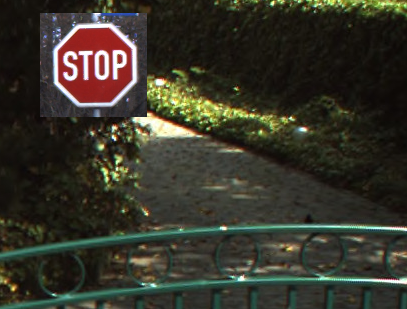
\includegraphics[width=0.49\linewidth]{images/stop_cropped.png}\hfill
    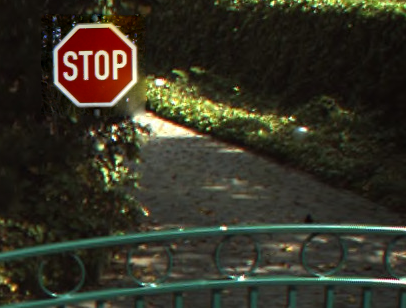
\includegraphics[width=0.49\linewidth]{images/stop_poisson.png}
    \caption{Porovnání vložení ořezané dopravní značky do pozadí. \textbf{Vlevo}: bez použitím techniky \emph{Poisson blending}. \textbf{Vpravo}: Po aplikaci techniky.}
    \label{fig:datasetCropped}
\end{figure}

\subsection{Použití transparentních značek}
V této metodě byly používány přesně ořezané dopravní značky malého počtu, obsahující alfa-kanál. Výhodou tohoto přístupu je, že kolem značky nevzniká přestupná hrana. Umisťování pouze tohoto malého počtu značek do pozadí by však způsobilo, že by se snímky začaly velmi brzy opakovat, a proto je před vložením do snímku provedena jejich syntetická úprava pomocí různých \emph{efektů}. Při aplikaci efektů je důležité, aby zůstal zachován realistický vzhled značek. Jednotlivé efekty lze vidět na obrázku \ref{fig:stopImplementace}.
Pravděpodobnost, s jakou se daný efekt aplikuje, i rozsah aplikovaných hodnot byly pečlivě vybírány a upravovány jak pomocí iterativně vyhodnocovaných experimentů (změny pravděpodobnosti aplikace a aplikovaných hodnot), tak inspirací vzhledu značek z reálného světa. Počet aplikovaných efektů na jednu značku není omezen. Výsledek lze vidět na obrázku \ref{fig:datasetTransparent}.
%Ani při dosažení realistického vzhledu (pro člověka) není jisté, zda se dokáže neuronová síť naučit potřebné vlastnosti a dokáže poté správně generalizovat na reálných snímcích, proto bylo potřeba provést řadu experimentů a iterativně generování zlepšovat.

\begin{figure}[t]\centering
    \centering
    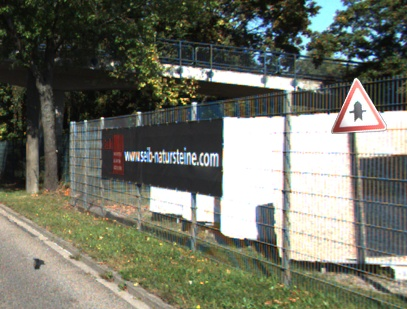
\includegraphics[width=0.49\linewidth]{images/synt_junction.png}\hfill
    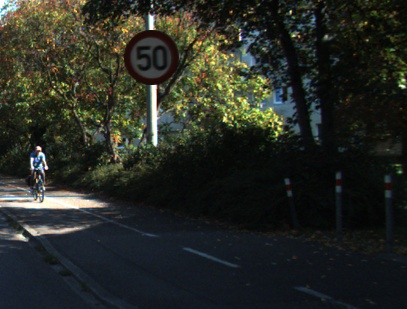
\includegraphics[width=0.49\linewidth]{images/synt_50.jpg}
    \caption{Příklad vygenerovaných dat (s různými světelnými podmínkami) pomocí transparentních značek a aplikace efektů upravujících vzhled značky.}
    \label{fig:datasetTransparent}
\end{figure}

\begin{figure}[t]\centering
    \centering
    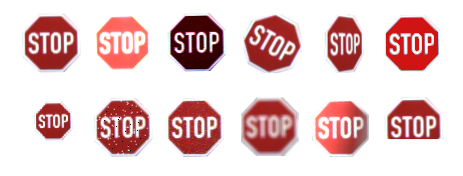
\includegraphics[width=0.99\linewidth]{images/znacky.png}
    \caption{Aplikace všech efektů používaných generátorem datových sad na značce typu \emph{stop}, vyřezané z reálného snímku. Originál vlevo nahoře.}
    \label{fig:stopImplementace}
\end{figure}

%Techniky, které naopak snížily úspěšnost modelu zahrnovaly například umisťování značek pouze na okraje silnic, a to tak že čím blíže byly středu, tím menší měli velikost (simulace reálného prostředí). Tyto pokusy však neprokázaly zvýšení úspěšnosti. Přidání luminiscenční podkladu a ocelové konstrukce značky měly za úkol přidat přirozený kontext, ve kterém se značky nachází, avšak výrazně snižovaly úspěšnost detekce. Jedna z vlastností značek je, že jsou osově souměrné, a proto byla vyzkoušena také rotace značek kolem osy \emph{y} (kromě značek obsahující šipky vlevo/vpravo apod.), ale úspěšnost se výrazněji nezměnila.


%--------------------------------------------------------
%--------------------------------------------------------
%--------------------------------------------------------
%--------------------------------------------------------
%--------------------------------------------------------

\section{Trénování detektoru značek}
Před samotným trénováním je důležité provést nastavení neuronové sítě pomocí konfiguračního souboru. V tomto souboru lze nastavit následující hodnoty. Počet filtrů, udávající počet konvolučních jader v dané vrstvě (nastaveno na \texttt{filters = (classes + 5) * 3}). Aktivační funkce, v téměř všech konvolučních vrstvách byla použita \emph{Leaky ReLu}, ve zbylých dvou (před \emph{yolo} vrstvami) lineární. Pokud je hodnota \texttt{random} nastavena na $1$ (použito vždy), mění daná vrstva náhodně velikost snímku. Důležitá je velikost vstupní vrstvy -- čím větší, tím lepších výsledků detekce bylo dosaženo, ale také se prodloužila doba detekce, jak lze vidět v porovnání na obrázku \ref{fig:porovnaniMapMs}. Další hodnoty jako např. velikost dávky, velikost kotev, masky, apod.

\subsection{Datová sada}
Pro trénování na syntetických datech bylo potřeba zjistit optimální počet generovaných značek na třídu. V tabulce \ref{tab:pocetSnimkuUspesnost} lze vidět závislost počtu syntetických snímků na výsledné úspěšnosti. Jak lze z tabulky vyčíst, mezi $200$, $500$ a $1000$ snímky se vyskytují velké skoky v úspěšnosti, zatímco mezi $1000$ a $2000$ se úspěšnost již téměř nezvýšila, zato se razantně prodloužila doba trénování. Jako optimální počet pro budoucí trénování na syntetických datech tedy vyšlo $1000$ značek na třídu. V případě trénování na reálných datech byla síť vždy trénována na $2/3$ počtu snímků z Belgické sady.

\begin{table}[h]
	\vskip6pt
	\caption{Závislost úspěšnosti YOLOv3-608 na množství syntetických snímků na třídu.}
	\centering
	\begin{tabular}{cc}
		\toprule
		Počet snímků & Úspěšnost v mAP\\
		\midrule
		$200$  & 63.2\% \\
		$500$  & 77.9\% \\
		\textbf{1000} & 86.3\% \\
		$2000$ & \textbf{87.6}\% \\
		\bottomrule
	\end{tabular}
	\label{tab:pocetSnimkuUspesnost}
\end{table}

\subsection{Experimenty}
Poté co bylo dosaženo dobré úspěšnosti a nedařilo se ji zvýšit za pomoci standardních metod, nastal čas provést řadu experimentů, které by mohly zajistit lepší parametry výsledného modelu.

\subsubsection*{Smíchání reálné se syntetickou datovou sadou}
Při trénování pouze na syntetické datové sadě se může konvoluční síť naučit vlastnosti vyskytující se pouze u syntetických snímků a nedokázat poté správně generalizovat na reálných snímcích. Proto bylo provedeno několik pokusů s přimícháním malého počtu reálných snímku k syntetické datové sadě. Tato malá sada reálných snímků by měla ``usměrňovat'' trénování správným směrem a výsledný model by poté měl dosáhnout lepší úspěšnosti na reálných snímcích. Při přidání cca. $30$ reálných snímků k $1000$ syntetickým snímkům na třídu došlo ke zvýšení mAP o 2\%.

\subsubsection*{Hard negative mining}
\emph{Hard negative mining} je technika postupného doplňování trénovací datové sady snímky, ve kterých bylo chybně interpretováno pozadí jako některý z detekovaných objektů.
%YOLO je trénováno na plných snímcích, kde detekované objekty tvoří velmi malou část z celého snímku a zbytek celého snímku se dá považovat za tzv. negativní datatovou sadu.
Po provedení několika testů se ukázalo, že ačkoli došlo ke snížení počtu falešně pozitivních detekcí, což bylo cílem, snížil se i počet správných detekcí a úspěšnost klesla o 3.5\% mAP z důvodů přetrénování.

\subsubsection*{Binární model}
Model XNOR-net pracuje jak se vstupem, tak s vahami ve formě binárních čísel. Tento model se používá pro zvýšení rychlosti na CPU a snížení výpočetních nároků, například pro použití v přenosných zařízeních s omezenými zdroji. Při testování s uvedeným modelem došlo k poklesu mAP o více než 20\% oproti běžnému modelu pracujícími s reálnými čísly a nevýraznému zvýšení rychlosti detekce.

\subsubsection*{Přidání dalších vrstev do architektury}
V modelu Tiny YOLOv3 se vyskytují dvě vrstvy \texttt{[yolo]} s kotvami. Protože značky mohou nabývat různých velikostí, pokusem bylo přidání třetí takovéto vrstvy s \texttt{mask = 6,7,8} (používající největší \emph{kotvy}) do modelu Tiny. Výsledkem byla úspěšnost obdobná modelu se dvěma vrstvami. Důvodem pravděpodobně bylo, že se v Belgické datové sadě nevyskytuje mnoho velkých značek, které by tato vrstva detekovala.

\subsubsection*{Přepočítání kotev}
\emph{Recalculate anchors}, tedy přepočítání ``kotev'', slouží k výpočtu nových hodnot tak, aby co nejlépe odpovídaly velikosti vstupních snímků. Tato technika má zvýšit průměrné \emph{IoU}, tzn. zajistit lepší úspěšnost detekce. Při přepočítání kotev na velikost vstupních snímků došlo ke zlepšení o 0.5\% mAP.

\subsubsection*{Počáteční hodnoty modelu}
Autoři systému poskytují několik před-trénovaných vah pro různé modely. Tyto váhy byly před-trénovány na datové sadě \emph{ImageNet} a protože konvoluční síť musí detekci hran a tvarů umět, je lepší využít již před-trénované hodnoty. Při použití před-trénovaných vah dosáhl výsledný model o cca. 2\% lepší mAP a při trénování potřeboval o 2000 iterací méně, než při trénování modelu od ``nuly''. Z tohoto důvodu byly při každém dalším trénování použity před-trénované váhy.

%--------------------------------------------------------
%--------------------------------------------------------
%--------------------------------------------------------
%--------------------------------------------------------
%--------------------------------------------------------

\section{Vyhodnocení}
\label{vyhodnoceniSekce}
Pro vyhodnocení úspěšnosti modelů byla použita metrika mAP (\emph{mean average precision}) s $IoU > .5$. Ta udává střední hodnotu AP všech tříd, kde AP je definováno jako plocha pod \emph{precision-recall} křivkou. \emph{Precision} (udávající jak přesné predikce jsou) na ose \emph{y} a \emph{recall} (udávající kolik ze všech pozitivních případů bylo správně predikováno) na ose \emph{x}~\cite{mAP}.

Při trénování modelu na reálná data byla Belgická datová sada rozdělena na dvě části. Větší částí sady bylo provedeno trénování modelu a na zbytku provedeno vyhodnocení. Trénování na syntetických datech umožnilo použít celou Belgickou datovou sadu pouze pro vyhodnocení úspěšnosti.


\subsection{Kvalitativní vyhodnocení}
Pokud je značka dobře viditelná a bez znatelného poškození, model ji ve většině případů správně detekuje s 90-100\% jistotou. Problém modelu dělají značky velmi malé, pod velkým úhlem, poničené či vybledlé, a také občasná záměna pozadí za objekt (pokud má objekt podobný tvar a barvu), jak lze vidět na obrázku \ref{fig:spatneDetekce}. Selhání potlačení nemaximálních hodnot, tzn. některá ze značek je detekována vícekrát, je nejméně často se vyskytující chybou, většinou pouze pokud je značka velmi blízko kameře. I přes to, že má YOLO problémy s dokonalou lokalizací objektů, predikované boxy ve většině případů ohraničují celou značku a to velmi přesně. Příklad několika detekcí za zhoršených podmínek lze vidět na obrázku \ref{fig:spravneDetekce}.

\begin{figure}[t]\centering
    \centering
    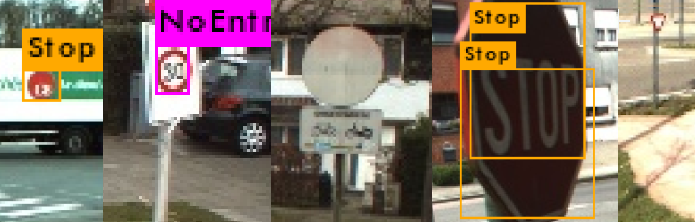
\includegraphics[width=0.99\linewidth]{images/spatne_detekce.png}
    \caption{Příklad často se vyskytujících nesprávných (falešně positivních) či chybějících (falešně negativních) detekcí.}
    \label{fig:spatneDetekce}
\end{figure}

\begin{figure}[t]\centering
    \centering
    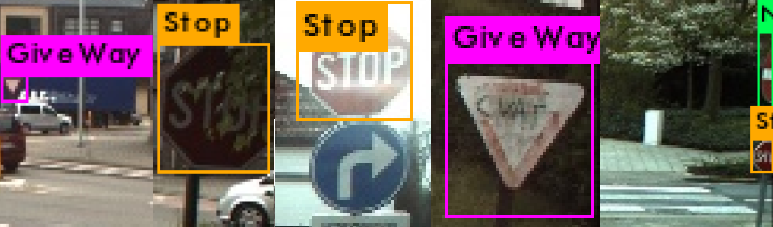
\includegraphics[width=0.99\linewidth]{images/spravne_detekce.png}
    \caption{Správné detekce i za zhoršených podmínek, jako například částečné překrytí značky, malá velikost, poškození a nevhodné světelné podmínky.}
    \label{fig:spravneDetekce}
\end{figure}


\subsection{Kvantitativní vyhodnocení}
K vyhodnocení úspěšnosti jsem využil repozitář \emph{mAP}~\cite{mAP_repo}, který jsem doplnil o vykreslení ROC (\emph{Receiver operating characteristic}) křivky a analýzu chyb.

\begin{figure}[t]\centering
    \centering
    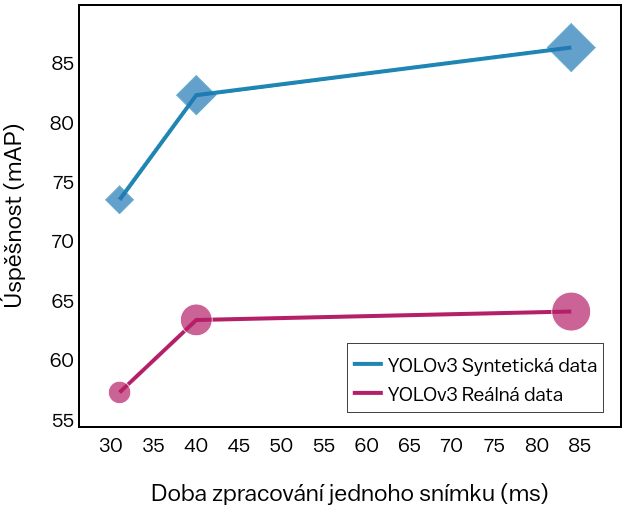
\includegraphics[width=0.99\linewidth]{images/map_ms_tradeoff.png}
    \caption{Porovnání závislosti úspěšnosti na době zpracování jednoho snímku třech modelů (zleva) YOLOv3-320, YOLOv3-416 a YOLOv3-608 trénovaných na syntetických a reálných datech. Zvětšující se velikost bodů reprezentuje velikosti vstupní vrstvy modelů. Z grafu lze vidět, že čím větší vstupní vrstva se použije, tím lepších výsledků detekce je dosaženo, ale také se tím prodlouží doba detekce. Za nejvhodnější lze tedy považovat prostřední model YOLOv3-416, který poskytuje nejlepší kompromis (tzv. \emph{tradeoff}) mezi úspěšností a časem. Výsledky byly získány na GeForce 840M.}
    \label{fig:porovnaniMapMs}
\end{figure}

\begin{figure*}[t!]\centering
    \centering
    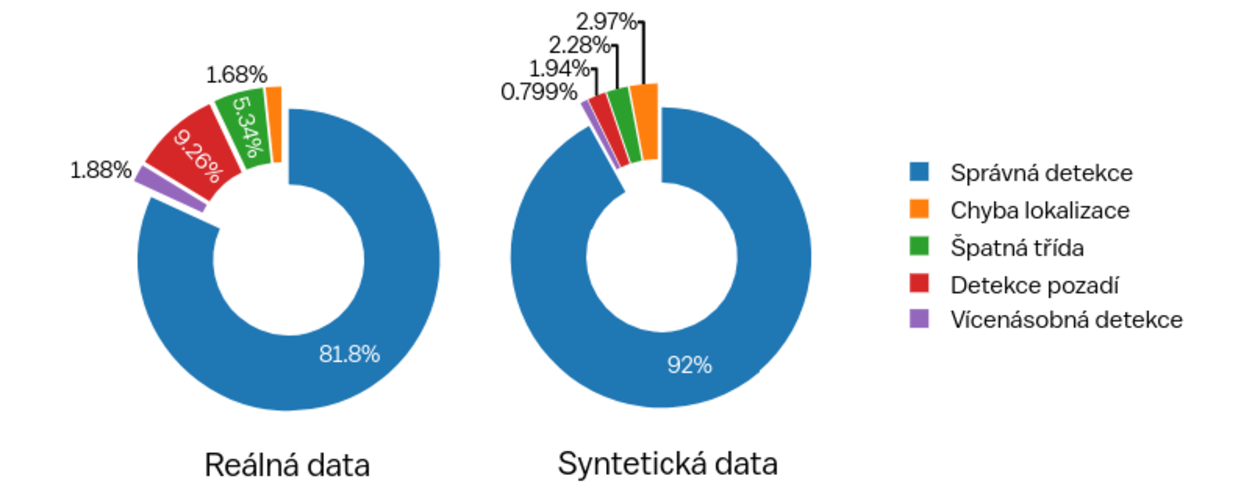
\includegraphics[width=0.90\linewidth]{images/error_analysis.pdf}
    \caption{Analýza chyb dvou modelů, trénovaných na reálných a syntetických datech. Model trénovaný na reálných datech (\textbf{vlevo}) má větší problém se záměnou pozadí s objekty a také nesprávné určování tříd značek. To je zapříčiněno nedostatečným množstvím informací o  některých třídách (malou velikostí datové sady). Naopak má nižší chybovost lokalizace, což znamená že dokáže predikované boxy lépe zarovnat na detekovanou značku. Pokles v úspěšnosti mAP zapříčiňují také falešně negativní vzorky, které do grafu nejsou zahrnuty.}
    \label{fig:analyzaChyb}
\end{figure*}

Výsledné modely měly poměrně vysoký počet falešně pozitivních predikcí, proto bylo vhodné zjistit, co dělá systému problém. Poté bylo možné navrhnout řešení a dosahovat tak lepších výsledků. Použil jsem metodiku analýzy chyb popsanou v práci~\cite{errorAnalysis}. Predikce je buď to správná, nebo je zařazena do jedné z následujících tříd~\cite{yolov1}.

\begin{itemize}
    \item \textbf{Správná predikce} -- správná třída, IoU $> 0.5$
    \item \textbf{Chyba lokalizace} -- správná třída, $\text{IoU} \in \interval({.1,.5})$
    \item \textbf{Podobné} -- podobná třída, $\text{IoU} > .1$
    \item \textbf{Ostatní} -- nesprávná třída, $\text{IoU} > .1$
    \item \textbf{Detekce pozadí} -- jakákoli detekce s $\text{IoU} < .1$
\end{itemize}

Více-násobná detekce jednoho objektu se dá také považovat za chybu (selhání potlačení nemaximálních hodnot), a proto bylo vyhodnocení doplněno o třídu vícenásobné detekce. Naopak kvůli nedostatku času nejsou detekce nesprávných tříd rozděleny do kategorií \emph{podobné} a \emph{ostatní}. Vizualizovanou distribuci chyb obou modelů lze vidět na obrázku \ref{fig:analyzaChyb}.

%--------------------------------------------------------
%--------------------------------------------------------
%--------------------------------------------------------
%	Podekovani
%--------------------------------------------------------
%--------------------------------------------------------
\section{Shrnutí}
Práce měla za úkol použít moderní architekturu konvoluční neuronové sítě pro detekci dopravních značek za účelem získání dobrých výsledků detekce v kombinaci s co možná nejkratší dobou zpracování. Dále bylo cílem vytvořit generátor syntetických datových sad a provést porovnání modelů trénovaných na reálných a syntetických datech a zjistit, zda jsou syntetická data pro podobné účely vhodná.

Nejlepším výsledkem získaným při trénování modelu na reálných datech bylo \textbf{63.4}\% mAP. Použití syntetických dat přineslo podstatně lepší úspěšnost detekce \textbf{82.3}\% mAP. Oběma modelům trvá vyhodnocení jednoho snímků v průměru \textbf{40.4}\emph{ms} na průměrně výkonném grafickém čipu Nvidia GeForce 840M. Při testování vyhodnocení na sdíleném clusteru s grafickým čipem Nvidia GTX 1080 Ti byla výsledná doba v průměru \textbf{3.9}\emph{ms} a na CPU Intel i5 bylo dosaženo průměrné rychlosti \textbf{1263}\emph{ms}.

Přínosem této práce je skutečnost, že ačkoli syntetická data nejsou pro trénování konvolučních sítí lepší než reálná, lze pomocí nich dosáhnout kvalitních výsledků bez nutnosti anotace tisíce snímků. Dále bylo potvrzeno, že Tiny YOLO třetí verze sice nedosahuje nejlepších výsledků detekce, ale zato velmi vysoké rychlosti zpracování snímků, což ze systému dělá zaslouženého konkurenta \emph{state of the art} metod.

V budoucnu by bylo možné rozšířit generátor datových sad o 3D analýzu pozadí a dopravních značek, za účelem dosažení vyšší realističnosti syntetické datové sady a hlubší analýzu trénování na syntetická data obecně. Vzhledem k faktu, že YOLO má problém s detekcí malých objektů, bylo by vhodné provést podobné porovnání detekce značek i u ostatních metod (SSD, Faster RCNN, apod.).

%--------------------------------------------------------
%--------------------------------------------------------
%--------------------------------------------------------
%	Podekovani
%--------------------------------------------------------
%--------------------------------------------------------
\section{Poděkování}
Zde bych rád poděkoval svému vedoucímu práce prof. Ing. Adamu Heroutovi, Ph.D za cenné rady, podnětné připomínky a vstřícnost při konzultacích. Dále za přístup k výpočetním a úložným zařízením ve vlastnictví stran a projektů, přispívajících k Národní Infrastruktuře Metacentrum v rámci programu "Projects of Large Research, Development, and Innovations Infrastructures" (CESNET LM2015042).

%--------------------------------------------------------
%--------------------------------------------------------
%--------------------------------------------------------
%	REFERENCE LIST
%--------------------------------------------------------
%--------------------------------------------------------
\phantomsection
\bibliographystyle{unsrt}
\bibliography{2019-ExcelFIT-detekceZnacek.bib}

%--------------------------------------------------------
%--------------------------------------------------------
%--------------------------------------------------------
\end{document}